\subsection{Android Studio}
Android Studio es el entorno de desarrollo integrado oficial para el 
desarrollo de aplicaciones para android, esta basado en IntelliJ IDEA~\cite{INTELLIJ}.

Además del potente editor de códigos y las herramientas 
para desarrolladores de IntelliJ, Android Studio ofrece aún
 más funciones que aumentan tu productividad durante la
 compilación de apps para Android, como las siguientes:

\begin{enumerate}
\item Un sistema de compilación basado en Gradle flexible.
\item Un emulador rápido con varias funciones.
\item Un entorno unificado en el que puedes realizar
 desarrollos para todos los dispositivos Android.
\item Instant Run para aplicar cambios mientras 
tu app se ejecuta sin la necesidad de compilar un nuevo APK.
\item Integración de plantillas de código y GitHub
 para ayudarte a compilar funciones comunes de las
 apps e importar ejemplos de código.
\item Gran cantidad de herramientas y frameworks
 de prueba.
\item Herramientas Lint para detectar problemas de
 rendimiento, usabilidad, compatibilidad de versión, etc.
\item Compatibilidad con C++ y NDK.
\item Soporte incorporado para Google Cloud Platform,
 lo que facilita la integración de Google Cloud Messaging 
y App Engine.
\end{enumerate}
\subsubsection{Interfaz de usuario}
La ventana principal de Android Studio consta 
de varias áreas lógicas que se identifican en la siguiente figura.
\linebreak 
\begin{figure}[h]
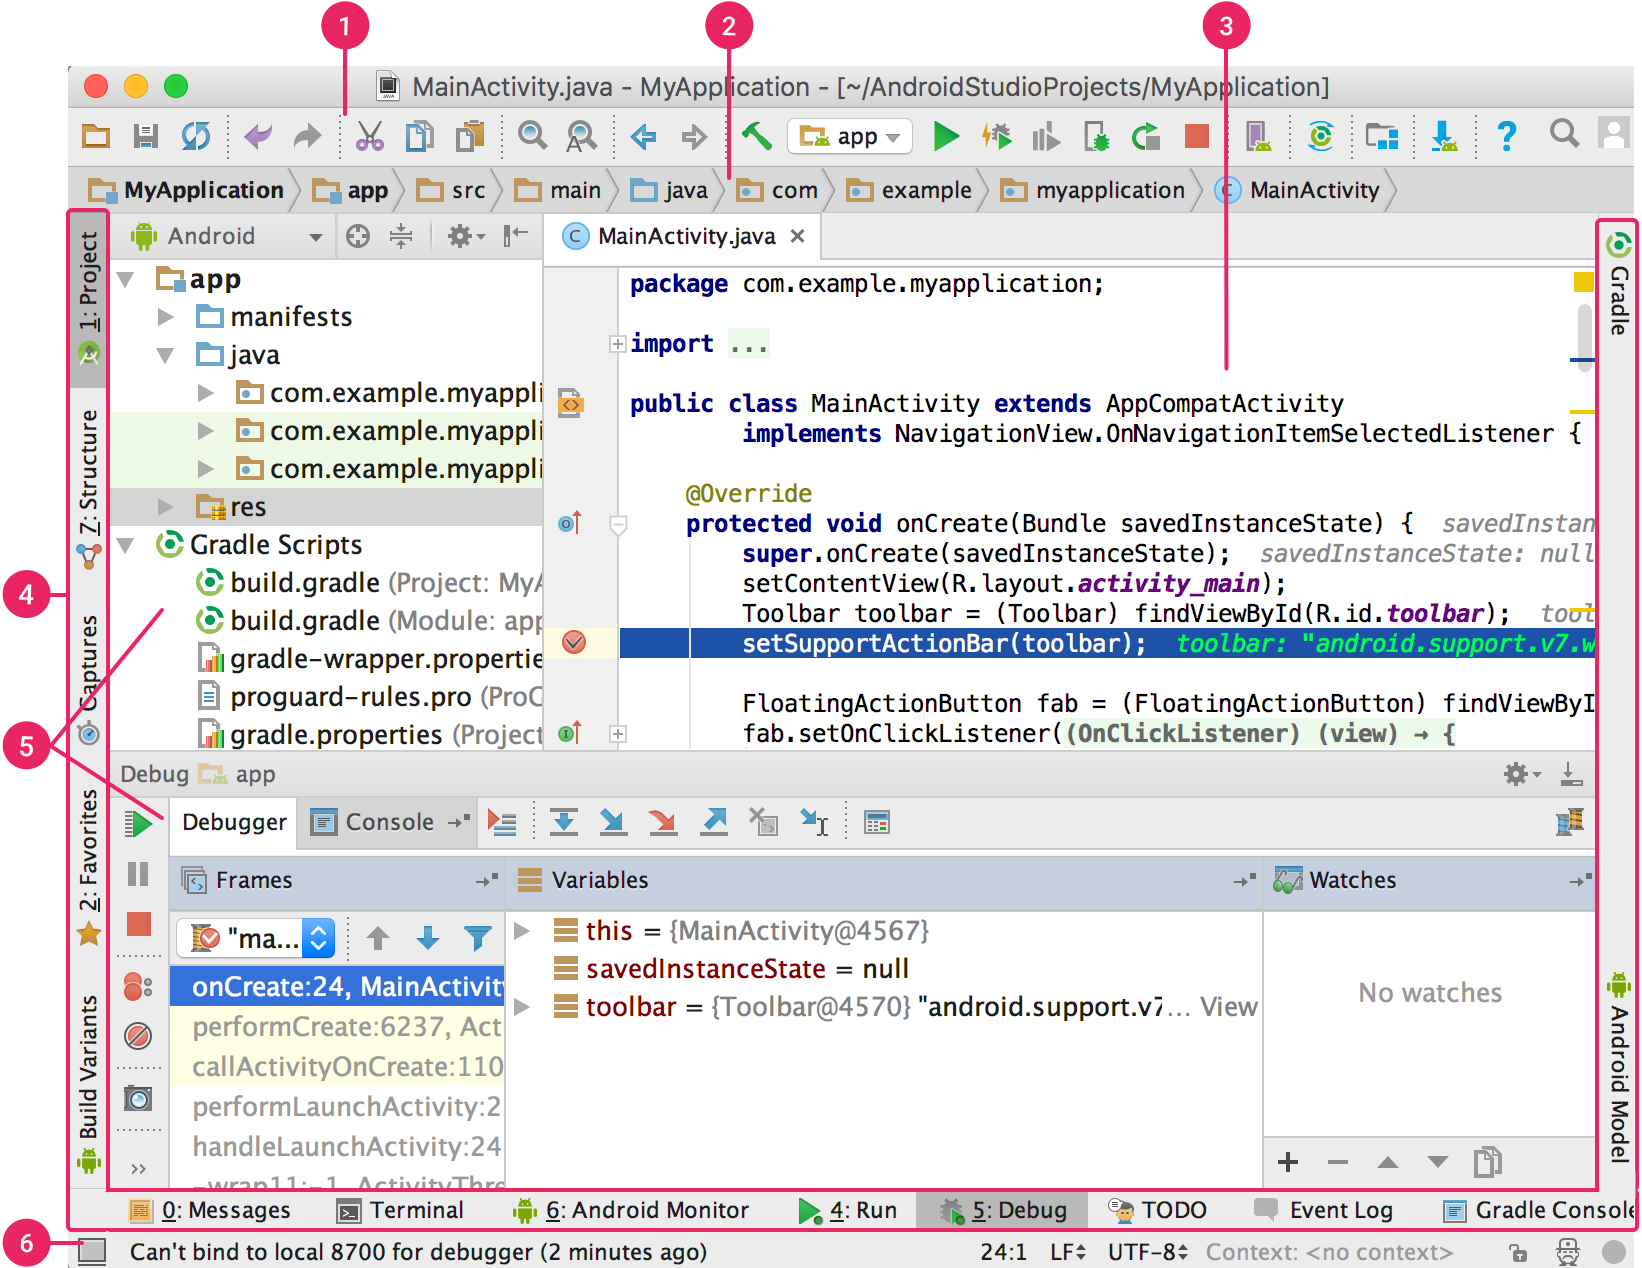
\includegraphics[scale=0.21]{ventana_android_studio.png} 
\caption{Ventana de Android Studio.}
\end{figure}

\begin{enumerate}
\item La barra de herramientas te permite realizar una gran
 variedad de acciones, como la ejecución de tu app y el inicio
 de herramientas de Android.
\item La barra de navegación te ayuda a explorar tu 
proyecto y abrir archivos para editar. Proporciona una 
vista más compacta de la estructura visible en la ventana Project.
\item La ventana del editor es el área donde puedes 
crear y modificar código. Según el tipo de archivo actual,
 el editor puede cambiar. Por ejemplo, cuando se visualiza
 un archivo de diseño, el editor muestra el editor de diseño.
\item La barra de la ventana de herramientas se extiende 
alrededor de la parte externa de la ventana del IDE y 
contiene los botones que te permiten expandir o contraer
 ventanas de herramientas individuales.
\item Las ventanas de herramientas te permiten acceder a 
tareas específicas, como la administración de proyectos,
 las búsquedas, los controles de versión, etc. Puedes 
expandirlas y contraerlas.
\item En la barra de estado, se muestra el estado de tu 
proyecto y del IDE en sí, como también cualquier advertencia 
o mensaje.
\end{enumerate}
\footnote{Fuente: Android Studio~\cite{ANDROIDSTUDIO}}